%%%%%%%%%%%%%%%%%%%%%%%%%%%%%%%%%%%%%%%%%
% Compact Laboratory Book
% LaTeX Template
% Version 1.0 (4/6/12)
%
% This template has been downloaded from:
% http://www.LaTeXTemplates.com
%
% Original author:
% Joan Queralt Gil (http://phobos.xtec.cat/jqueralt) using the labbook class by
% Frank Kuster (http://www.ctan.org/tex-archive/macros/latex/contrib/labbook/)
%
% License:
% CC BY-NC-SA 3.0 (http://creativecommons.org/licenses/by-nc-sa/3.0/)
%
% Important note:
% This template requires the labbook.cls file to be in the same directory as the
% .tex file. The labbook.cls file provides the necessary structure to create the
% lab book.
%
% The \lipsum[#] commands throughout this template generate dummy text
% to fill the template out. These commands should all be removed when 
% writing lab book content.
%
% HOW TO USE THIS TEMPLATE 
% Each day in the lab consists of three main things:
%
% 1. LABDAY: The first thing to put is the \labday{} command with a date in 
% curly brackets, this will make a new section showing that you are working
% on a new day.
%
% 2. EXPERIMENT/SUBEXPERIMENT: Next you need to specify what 
% experiment(s) and subexperiment(s) you are working on with a 
% \experiment{} and \subexperiment{} commands with the experiment 
% shorthand in the curly brackets. The experiment shorthand is defined in the 
% 'DEFINITION OF EXPERIMENTS' section below, this means you can 
% say \experiment{pcr} and the actual text written to the PDF will be what 
% you set the 'pcr' experiment to be. If the experiment is a one off, you can 
% just write it in the bracket without creating a shorthand. Note: if you don't 
% want to have an experiment, just leave this out and it won't be printed.
%
% 3. CONTENT: Following the experiment is the content, i.e. what progress 
% you made on the experiment that day.
%
%%%%%%%%%%%%%%%%%%%%%%%%%%%%%%%%%%%%%%%%%

%----------------------------------------------------------------------------------------
%	PACKAGES AND OTHER DOCUMENT CONFIGURATIONS
%----------------------------------------------------------------------------------------                               

\documentclass[fontsize=11pt, % Document font size
                             paper=a4, % Document paper type
                             twoside, % Shifts odd pages to the left for easier reading when printed, can be changed to oneside
                             captions=tableheading,
                             index=totoc,
                             hyperref]{labbook}
 
\usepackage[bottom=10em]{geometry} % Reduces the whitespace at the bottom of the page so more text can fit

\usepackage[english]{babel} % English language
\usepackage{lipsum} % Used for inserting dummy 'Lorem ipsum' text into the template

\usepackage[utf8]{inputenc} % Uses the utf8 input encoding
\usepackage[T1]{fontenc} % Use 8-bit encoding that has 256 glyphs

\usepackage[osf]{mathpazo} % Palatino as the main font
\linespread{1.05}\selectfont % Palatino needs some extra spacing, here 5% extra
\usepackage[scaled=.88]{beramono} % Bera-Monospace
\usepackage[scaled=.86]{berasans} % Bera Sans-Serif

\usepackage{booktabs,array} % Packages for tables

\usepackage{amsmath} % For typesetting math
\usepackage{graphicx} % Required for including images
\usepackage{etoolbox}
\usepackage{fancyvrb}
\usepackage{float}
\usepackage[norule]{footmisc} % Removes the horizontal rule from footnotes
\usepackage{lastpage} % Counts the number of pages of the document
\usepackage{subcaption}
\let\theHsubfigure\relax
\usepackage[dvipsnames]{xcolor}  % Allows the definition of hex colors
\definecolor{titleblue}{rgb}{0.16,0.24,0.64} % Custom color for the title on the title page
\definecolor{linkcolor}{rgb}{0,0,0.42} % Custom color for links - dark blue at the moment

\addtokomafont{title}{\Huge\color{titleblue}} % Titles in custom blue color
\addtokomafont{chapter}{\color{OliveGreen}} % Lab dates in olive green
\addtokomafont{section}{\color{Sepia}} % Sections in sepia
\addtokomafont{pagehead}{\normalfont\sffamily\color{gray}} % Header text in gray and sans serif
\addtokomafont{caption}{\footnotesize\itshape} % Small italic font size for captions
\addtokomafont{captionlabel}{\upshape\bfseries} % Bold for caption labels
\addtokomafont{descriptionlabel}{\rmfamily}
\setcapwidth[r]{10cm} % Right align caption text
\setkomafont{footnote}{\sffamily} % Footnotes in sans serif

\deffootnote[4cm]{4cm}{1em}{\textsuperscript{\thefootnotemark}} % Indent footnotes to line up with text

\DeclareFixedFont{\textcap}{T1}{phv}{bx}{n}{1.5cm} % Font for main title: Helvetica 1.5 cm
\DeclareFixedFont{\textaut}{T1}{phv}{bx}{n}{0.8cm} % Font for author name: Helvetica 0.8 cm

\usepackage[nouppercase,headsepline]{scrlayer-scrpage} % Provides headers and footers configuration


\pagestyle{scrheadings} % Print the headers and footers on all pages
\clearscrheadfoot % Clean old definitions if they exist

\automark[chapter]{chapter}
\ohead{\headmark} % Prints outer header

\setlength{\headheight}{25pt} % Makes the header take up a bit of extra space for aesthetics
\setheadsepline{.4pt} % Creates a thin rule under the header
\addtokomafont{headsepline}{\color{lightgray}} % Colors the rule under the header light gray

\ofoot[\normalfont\normalcolor{\thepage\ |\  \pageref{LastPage}}]{\normalfont\normalcolor{\thepage\ |\  \pageref{LastPage}}} % Creates an outer footer of: "current page | total pages"

% These lines make it so each new lab day directly follows the previous one i.e. does not start on a new page - comment them out to separate lab days on new pages
\makeatletter
\patchcmd{\addchap}{\if@openright\cleardoublepage\else\clearpage\fi}{\par}{}{}
\makeatother
\renewcommand*{\chapterpagestyle}{scrheadings}

% These lines make it so every figure and equation in the document is numbered consecutively rather than restarting at 1 for each lab day - comment them out to remove this behavior
\usepackage{chngcntr}
\counterwithout{figure}{labday}
\counterwithout{equation}{labday}

% Hyperlink configuration
\usepackage[
    pdfauthor={}, % Your name for the author field in the PDF
    pdftitle={Cleaning and Mapping Robot Laboratory Journal}, % PDF title
    pdfsubject={}, % PDF subject
    bookmarksopen=true,
    linktocpage=true,
    urlcolor=linkcolor, % Color of URLs
    citecolor=linkcolor, % Color of citations
    linkcolor=linkcolor, % Color of links to other pages/figures
    backref=page,
    pdfpagelabels=true,
    plainpages=false,
    colorlinks=true, % Turn off all coloring by changing this to false
    bookmarks=true,
    pdfview=FitB]{hyperref}

\usepackage[stretch=10]{microtype} % Slightly tweak font spacing for aesthetics

%\setlength\parindent{0pt} % Uncomment to remove all indentation from paragraphs

%----------------------------------------------------------------------------------------
%	DEFINITION OF EXPERIMENTS
%----------------------------------------------------------------------------------------

% Template: \newexperiment{<abbrev>}[<short form>]{<long form>}
% <abbrev> is the reference to use later in the .tex file in \experiment{}, the <short form> is only used in the table of contents and running title - it is optional, <long form> is what is printed in the lab book itself

\newexperiment{example}[Example experiment]{This is an example experiment}
\newexperiment{example2}[Example experiment 2]{This is another example experiment}
\newexperiment{example3}[Example experiment 3]{This is yet another example experiment}

\newsubexperiment{subexp_example}[Example sub-experiment]{This is an example sub-experiment}
\newsubexperiment{subexp_example2}[Example sub-experiment 2]{This is another example sub-experiment}
\newsubexperiment{subexp_example3}[Example sub-experiment 3]{This is yet another example sub-experiment}

%----------------------------------------------------------------------------------------

\begin{document}

%----------------------------------------------------------------------------------------
%	TITLE PAGE
%----------------------------------------------------------------------------------------

\title{\textcap{Cleaning and Mapping Robot Laboratory Journal \\[1cm]  
\textaut{Beginning 5-27-2020}}}

\author{
    \textaut{Brian Lauer}\\ \\ % Your name
    \textaut{Nicolaus Shepard}\\ 
}
\date{} % No date by default, add \today if you wish to include the publication date

\maketitle % Title page

\printindex
\tableofcontents % Table of contents
\newpage % Start lab look on a new page

\begin{addmargin}[0cm]{0cm} % Makes the text width much shorter for a compact look

\pagestyle{scrheadings} % Begin using headers

%----------------------------------------------------------------------------------------
%	LAB BOOK CONTENTS
%----------------------------------------------------------------------------------------

\labday{Wednesday, May 27, 2020}
Problem Statement:\\
Various cleaning and mapping (CAM) robots such as the Roomba by iRobot are commercially available today and are able to clean different areas of a home or business. Some of the top of the line robots by iRobot like the Roomba s9+, Roomba i7+, and Braava m6 are able to map rooms with a technology called Imprint Smart Mapping technology. In the app for each robot, a clean map report can be generated\footnote{\url{https://homesupport.irobot.com/app/answers/detail/a_id/1467}}. The generated 2D map will show areas that were cleaned by the robot and the white areas that contained obstacles like furniture or appliances. In these robots that support the mapping feature, a camera is mounted at an angle of 45 degrees that takes pictures of a room regularly. These images are then processed using Visual Simultaneous Localization and Mapping (VSLAM)\footnote{\url{https://www.thezebra.com/resources/home/how-roomba-works/}}. Multiple alternative techniques for localization and mapping a robot including lidar and RFID technology. In the proposed research, RFID technology will be utilized for the purpose of possibly lowering costs and computational complexity.
\smallbreak\noindent
Research efforts:\\
In~\cite{hahnel2004}, a probabilistic model for localizing an RFID tag is given for the purpose of localizing a robot in its environment. Given a the position $x$ of the tag and data $z_{1:t}$, the probability of obtaining the correct position of the robot given the observations is 
\[
p(x|z_{1:t})=\alpha p(z_t \vert x) p(x \vert z_{1:t-1})
\]
where $\alpha$ is the normalization constant. The purpose of this study was to determine the locations of RFID tags in an office building using a laser range finder and an RFID reader mounted on the robot. With the RFID tag's locations the path of the robot could be estimated which is known as localization. However, it does not use RFID specifically for mapping an environment. Therefore, techniques must be found for determining how to map the robot's environment. This may only be possible with sensors like a laser range finder, LIDAR sensor, or other digital devices like a camera.

\labday{Thursday, May 28, 2020}
I received the resources for the iRobot Create 2 from Jaden today in his Google Drive. The iRobot Create 2 is a hackable device designed for education rather than commercial use\footnote{\url{https://www.irobot.com/About-iRobot/STEM/Create-2/Projects.aspx}}. On iRobot's site, many different projects have been done with this robot such as a Nerf-gun mounted turret modification, nerf-gun dart collector robot, camera bot, pokemon go egg hatching, zcm driver, and path finder. All of them are documented in the provided footnote.

\labday{Monday, June 1, 2020}
Today, I did some research on how to implement the mapping feature with a LIDAR sensor as Prof. Miah mentioned that this technology is available in some of the labs. I looked at a tutorial on how to interface the Neato LIDAR sensor with a Beaglebone~\footnote{\url{https://www.alexschimp.com/neato-lidar-data-beaglebone-black/}}. By simply connecting the LIDAR sensor to the TX and RX pins of the board, data can be sent to the device or the encoded can be retrieved. The mentioned LIDAR comes with a motor which can be powered with a $3$V power supply. To read from the device the device file in the \texttt{/dev} directory must be opened. Each packet consists of 22 bytes. The code below:
\begin{Verbatim}
print("Hello")

with open("/dev/ttyO2", "rb") as f:
    byte = f.read(1)
    count = 1
    while byte != "" and count <= 22*100:
        print(byte.encode('hex') + ":")
        byte = f.read(1)
        count += 1

print("Goodbye")
\end{Verbatim}
where the LIDAR is located at \texttt{/dev/tty02}. However, the LIDAR sensor that Prof. Miah has in his robotics lab is likely different as there are a lot of different options out there.

\labday{Tuesday, June 2, 2020}
In yesterday's meeting with Jaden, my partner, we agreed that he would focus mostly on the hardware side of things as he has the robot and beaglebone while I work on building an Android app for showing the map. In this way, I will be able to make more of a significant contribution toward the project with the resources I currently have. I have never built an app before so some research will be required before I start developing the app.
\smallbreak\noindent
I started by following the Android tutorial\footnote{\url{https://developer.android.com/training/basics/firstapp/creating-project}}. The UI for each app is built using a system of layouts and widgets where the layouts are \texttt{ViewGroup} objects and the widgets are \texttt{View} objects. Objects in the layout like text objects and buttons can be constrained to each other. For each TextView object, a \texttt{textSize} and \texttt{textColor} variable can be set. The result of the tutorial is shown below:
\begin{figure}[H]
\centering
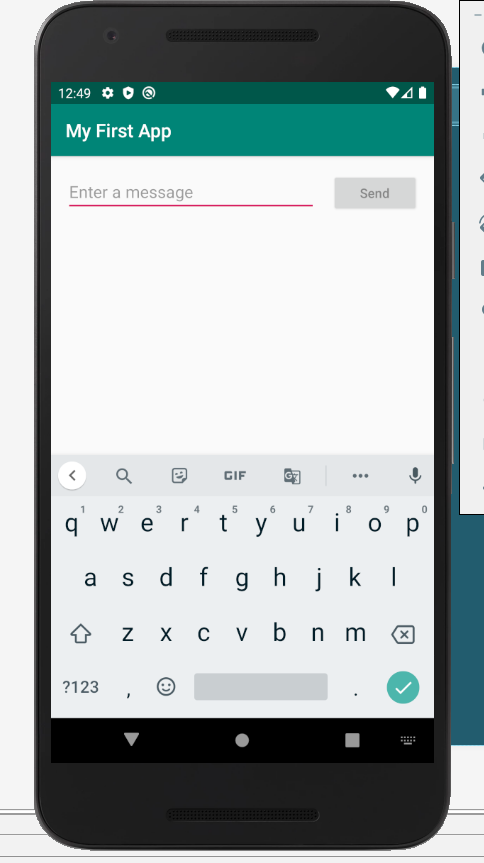
\includegraphics[scale=0.5]{figs/img/myFirstApp}
\end{figure}
where after text is entered and the button is pressed, a new activity is shown which displays the text under the top app bar.

\labday{Wednesday, June 3, 2020}
Today I took a pause on developing the app by looking at the link to the Lidar sensor that Dr. Miah sent us that is available in the robotics facility~\footnote{\url{https://www.robotshop.com/en/rplidar-s1-360-laser-scanner-40-m.html?utm_source=google&utm_medium=surfaces&utm_campaign=surfaces_across_google_usen&gclid=EAIaIQobChMI9JyBto7m6QIVkIbACh3GMwhZEAYYASABEgIebPD_BwE}}. 
The model is a RPiLIDAR S$1$ $360^\circ$. According to the datasheet it can perform 2D $360^\circ$ scan of an area with a 40 meter range. The sampling rate is 9200 samples per second and the sensor can tilt vertically up $0.391^\circ$. While scanning, the data output of the sensor over UART includes both the distance between the rotating LIDAR sensor and the sampling point while the heading is the current angle of measurement in degrees. A flag in the data will signal the start of a new scan. Both the distance and heading values will be sent as pairs for data communication for each sample point. The pinout for the device is as follows:

\begin{center}
\begin{tabular}{|c|c|}
\hline
Pin Name & Description \\
VCC & Power\\
GND & Power\\
RX & Serial Input\\
TX & Serial Output\\
\hline
\end{tabular}
\end{center}
where there are two pins for VCC and GND each as separate power is needed for the sensor and motor system that rotates the sensor. Because the connector used for the sensor is a SH$1.0$-$6$P, some special wires may be needed for connecting to the device. As far as the specification for the serial interface goes, the baud rate is 256000 bps and uses 3.3V TTL logic.
\smallbreak\noindent
Since I am on my laptop and do not have android studio installed on it, I began installing it. I realized that the Create 2 does not have any sort of internet connectivity, so a web server will be needed on the Beaglebone to communicate with it wirelessly. In the app, some functionality will need to be developed to discover the Roomba on the network. 
\smallbreak\noindent
I created a new project called LidarMap using the bottom navigation bar template.

\labday{Thursday, June 4, 2020}
I spent some time wireframing the UI for the app on paper today. The app will have a bottom navigation bar with the pages Discovery and Map. The Discovery page will contain the list of discovered robots while the Map page will contain the map similar to the map shown in the Roomba app. Similar to my building energy management project, the robots should be discovered automatically with an "autodiscovery" feature. While waiting for devices to be discovered I want to add an indefinite progress bar spinner. Since I realized that it is possibly going to be more difficult to change the current icons in the current app I decided that I will simply start making the app using a blank template.
\smallbreak\noindent
I thus created a new Android Studio project named \texttt{Create2LidarMap} using Android 4.0.3 (Ice Cream Sandwich) using the empty activity template. I then followed~\footnote{\url{https://androidwave.com/bottom-navigation-bar-android-example/}} to create a bottom nav bar from scratch. 

\labday{Friday, June 5, 2020}
I worked on adding the bottom navigation menu from scratch into the app. The icons were successfully added where one is a magnifying glass and the other is a quilt for the map page. The \texttt{NavHostFragment} component in the MainAcitity page will provide an area above the nav menu for self contained navigation to occur. Essentially two different fragments will be created for the discovery and map respectively. However after adding the component to the main activity and importing the Android jetpack package \texttt{androidx.navigation.fragment}, I got a warning stating that to Replace the tag With FragmentContainerView. I made the change to this View but another issue came up as the navGraph attribute excepts a resource of type String but currently has a navigation resource type (@navigation/mobile\_navigation). Inside the onCreate method in the \texttt{MainActivity} class, I added the line
\begin{Verbatim}
this.getSupportActionBar().hide();
\end{Verbatim}
To remove the top action bar with the name of the activity which in my opinion makes the app look a little cleaner.

\labday{Monday, June 8, 2020}
Because of the issues mentioned previously with adding the navbar from a blank project, I decided to simply take the original LidarMap project and modify it with the appropriate fragment and subtract and add the appropriate navbar elements. In the java directory I created a package\texttt{com.example.ui.lidarmap.map} where I created the java file \texttt{MapFragment.java} and \texttt{MapViewModel.java}. The source code for MapFragment was generated by default and contains the following:
\begin{Verbatim}
package com.example.lidarmap.ui.map;

import androidx.lifecycle.ViewModelProviders;

import android.os.Bundle;

import androidx.annotation.NonNull;
import androidx.annotation.Nullable;
import androidx.fragment.app.Fragment;

import android.view.LayoutInflater;
import android.view.View;
import android.view.ViewGroup;

import com.example.lidarmap.R;

public class MapFragment extends Fragment {

    private MapViewModel mViewModel;

    public static MapFragment newInstance() {
        return new MapFragment();
    }

    @Override
    public View onCreateView(@NonNull LayoutInflater inflater, 
    @Nullable ViewGroup container,
                             
                            @Nullable Bundle savedInstanceState) {
        return inflater.inflate(R.layout.map_fragment, container, false);
    }

    @Override
    public void onActivityCreated(@Nullable Bundle savedInstanceState) {
        super.onActivityCreated(savedInstanceState);
        mViewModel = ViewModelProviders.of(this).get(MapViewModel.class);
        // TODO: Use the ViewModel
    }

}
\end{Verbatim}
I created a second package named \texttt{com.example.lidarmap.ui.discovery} with the files \texttt{DiscoveryFragment} and \texttt{DiscoveryViewModel} which similar code to the map fragment and view model classes. After adding these files, I generated the layout files. However, the build failed with the exception: \texttt{java.lang.RuntimeException}. I thus decided to once again create a new project from scratch in hopes of fixing the previous issues from the \texttt{CAMRobotMap} project.
\smallbreak\noindent
I decided to scrap all my previous ideas and simply follow a tutorial on Youtube at \footnote{\url{https://www.youtube.com/watch?v=tPV8xA7m-iw}}. At the beginning of the tutorial, the speaker mentioned that if only two destinations are needed (map, discovery) then it is better to use a tab layout instead. I deleted the old project with the bottom nav and created a new project with tabbed activity template. Instead I decided the follow the tutorial \footnote{\url{https://www.youtube.com/watch?v=h4HwU_ENXYM}}. In the "Discovery" tab, I added a ListView object 

\labday{Wednesday, June 10, 2020}
What I plan on accomplishing today is creating a github repository for the android app and sharing with Jaden, so that we can both work on the software together as he cannot do much due to hardware limitations with the Roomba. Next I would like to start writing a method to create a TCP/UDP client and send out broadcast messages on the network for the Roomba. First, I asked Dr. Miah for permission before pushing the project to a public Github repository. However, I found that I recent change was made to github that allows for unlimited private repos with fewer than 3 or 4 collaborators. When attempting to the push the changes to the repository I got the error:
\begin{verbatim}
Push rejected: Push to origin/master was rejected
\end{verbatim}
This was fixed after I rebased from master to refs/remotes/origin/master. Thus, I was able to succesfully push the project to the github repo LidarMappingRobot.
\smallbreak\noindent
Although the priority is to write the TCP/IP client code for the app, I would like to add subitems into the list view for the Discovery fragment. 

\labday{Thursday, June 11, 2020}
\begin{figure}[H]
\centering
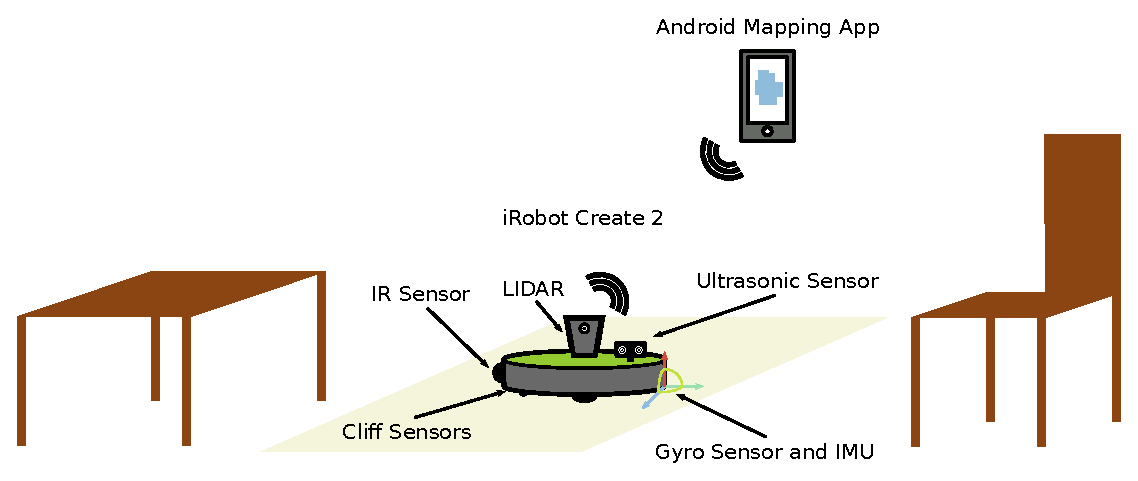
\includegraphics[scale=0.7]{figs/inkscape/mappingRobotArchitecture.eps}
\caption{Diagram representing the working principal of the cleaning and mapping robot}
\end{figure}
\noindent
Description:
\smallbreak
The proposed cleaning and mapping robot based off the Roomba vacuum by iRobot will have the ability to collect sensor data from multiple onboard sensors connected to a single board computer (Beaglebone Blue) for the purpose of localization and mapping. IR sensors, ultrasonic sensors, cliff sensors, and LIDAR will help the robot to understand its environment better. The IMU and gyroscope will help to track orientation, velocity, and rotation. With the aid of the computer, the robot will be able to successfully map its environment like a floor of a house or building. The LIDAR sensor will perform a continuous $360^\circ$ sweep of the environment to generate a $2$D map of the environment. For visualizing the fully completed map, an Android app will be developed to display the outcome of the mapping graphically. Built-in WiFi support of the Beaglebone will act as the communication medium between the robot and client. iRobot has developed a technology of their own that can perform mapping of an area and identify areas of high dirt or dust concentration. However, the robot to be developed will seek to use cost effective sensors to clean the floor and build a map of the environment. The robot will exhibit human like reasoning and intelligence including perception and memory through storage of maps on the single board computer. Techniques like artificial intelligence will be deployed for improving the human like perception abilities of the device even further. 

\labday{Tuesday, June 16, 2020}
Brian:
I found a blog post on the Internet detailing how to implement a network scanning feature in Android\footnote{\url{https://cheesecakelabs.com/blog/developing-iot-apps-connecting-smart-devices/}}. At the end of section 1, it states that networking code should not run in the UI. In other words, a separate thread of execution must be created for network operations. In this case, scanning all IP addresses on a subnet is the task at hand. I worked on understanding the method \texttt{getIpv4Netmask()} which should return the network prefix length or in other words the number of bits in the network portion of the IP address. However I tried the code out in Eclipse and received a \texttt{NullPointerException}. This may have to do with passing the wrong IP address as a parameter into the method call. To try and understand what IP address should be passed in an argument, I used the lines
\begin{Verbatim}
WifiManager wifiManger = (WifiManager) getSystemService(Context.WIFI_SERVICE);
DhcpInfo dhcpInfo = wifiManger.getDhcpInfo();
\end{Verbatim}
in the \texttt{onCreate} method of the \texttt{MainActivity} class. However, the  \texttt{getDhcpInfo} call was returning an error as the WifiManager is missing permissions. What I found is that the permission \texttt{ACCESS\_WIFI\_STATE} is required in the Android Manifest file which is accomplished by adding the line.
\begin{Verbatim}
<uses-permission android:name="android.permission.ACCESS_WIFI_STATE" />
\end{Verbatim}
to the AndroidManifest.xml file. Also, I changed the lines to 
\begin{Verbatim}
WifiManager wifiManager = (WifiManager) getContext().getApplicationContext()
.getSystemService(Context.WIFI_SERVICE);
DhcpInfo dhcpInfo = wifiManager.getDhcpInfo();
\end{Verbatim}
As a test, since the wifi is not enabled on the emulator, I downloaded the app to a test Moto E phone. An added \texttt{dhcpInfo.ipAddress} to the the list of items. It displays the integer $318810304$ which by using a decimal to IP converter I found the this represents the IP address 192.168.0.19.

\labday{Wednesday, June 17, 2020}
Since I was having problems with finding the prefix length with the getIpv4Netmask provided in the footnote above, I decided to rather get the localhost of the device and get the network interfaces attached. In this way, hopefully a null reference exception will be avoided. Unfortunately, when I call \texttt{Inet4Address.getLocalHost()} the app crashes. I found that this is caused by a \texttt{NetworkOnMainThreadException} being thrown by the application as it was trying to perform a network operation on the main thread. I did not realize that it is absolutely required to add in a second thread to perform network operations. 
\smallbreak\noindent
I need to create another class in the \texttt{DiscoveryFragment} class that extends from the \texttt{AsyncTask} class. However, I discovered that the \texttt{AsyncTask} class was deprecated in API level 30. Instead I will use the more up to date \texttt{Executor} interface which contains one method: \texttt{execute}. In the implementation of the the \texttt{execute} method, it creates a new thread and starts it as follows:
\begin{Verbatim}
class TaskExecutor implements Executor {
	public void execute(Runnable r) {
		new Thread(r).start();
	}
}
\end{Verbatim}
Where \texttt{Runnable} is a second interface that adds the \texttt{run} method which will be executed when the thread is started. In the \texttt{run} method, I would like to get the network prefix of the subnet and add to the ArrayList to be added to the ListView in the android application. 
\smallbreak\noindent
This second issue to be solved is the issue of the \texttt{getLocalHost} method returning a \texttt{InetAddress} object bound to the IP address 127.0.0.1 rather than the actual address of the device. The network mask prefix of 127.0.0.1 is 8 rather than the expected 24 on my home network. After implementing some more of the code by using an instance of the DhcpInfo object, I was able to successfully display the prefix (24) in the app.

\labday{Thursday, June 18, 2020}
Today will be detected to searching for all devices under my networks subnet (255.255.255.0). I created a second task titled \texttt{ScanNetworkTask}. However, I would like to write a method that will be called in the \texttt{ScanNetworkTask} run method for obtaining the network prefix rather than using a separate thread to find the prefix. The purpose for doing this is to prevent a race condition with the class level member variable \texttt{mNetworkPrefix}. The problem I am having is that private member variables cannot be accessed from static methods in java. The variable I would like to reference is the instance of \texttt{DhcpInfo} which is initialized in the \texttt{onCreate} method of the \texttt{DiscoveryFragment} class. However, in the end, I just decided to add all the code including the code to determine the network prefix in a single task class titled \texttt{ScanSubnetTask}. The code after the network prefix code will loop from 192.168.0.0 up to 192.168.0.254 and ping each of those addresses by calling the \texttt{InetAddress.isReachable} method with a timeout of 80 ms. In the task, I decided to update the ArrayList with the list of reachable IP addresses. This causes an \texttt{IllegalStateException} because the background thread should not be sending notifications to the UI to update it. Correctly communicating with the UI from backgrounds will be necessary here \footnote{\url{https://developer.android.com/training/multiple-threads/communicate-ui}}.

\labday{Friday, June 19, 2020}
Today, I read through some of the android developer resources to determine how to update the UI from a background thread. A line that I found that should be added to the implementation of the \texttt{run} method is
\begin{Verbatim}
android.os.Process.setThreadPriority(android.os.Process.THREAD_PRIORITY_BACKGROUND);
\end{Verbatim}
which moves the thread to the background. Inside the constructor of the \texttt{DiscoveryFragment} class I added an instance of an anonymous class which extends the \texttt{Handler} class will handle new message added to the task:
\begin{Verbatim}
    private DiscoveryFragment() {
        // This is an anonymous class which extends the Handler class
        handler = new Handler(Looper.getMainLooper()) {
            @Override
            public void handleMessage(Message inputMessage) {

            }

        };
    }
\end{Verbatim}
The problem is I don't know how the invoke the handler and what type of message will be passed into the \texttt{handleMessage} method. It turns out the \texttt{sendMessage} method must be used. From the android developer docs \footnote{\url{https://developer.android.com/reference/android/os/Message}}, the \texttt{Message} class is used to define a message containing a description and data object to be sent to a handler. The \texttt{setData} must be called on an instance of the Message object in order to add data to the Message instance. When attempting to call the \texttt{sendMessage} method on the handler instance, I received the following exception:
\begin{Verbatim}
java.lang.IllegalStateException: 
{ when=-14h27m43s520ms what=0 
target=com.example.lidarmappingrobot.ui.main.DiscoveryFragment$1 } 
This message is already in use.
\end{Verbatim}
%$

\labday{Monday, June 22, 2020}
One of the problems I discovered in my code, is that the \texttt{Message.sendMessage(Message)} method was being called inside a for loop. Thus, the same \texttt{Message} object was likely being used multiple times causing some issues. After adding the \texttt{sendMessage} call after the for loop the exception went away. However, no IP addresses were being listed in the Discovery page. Instead of assigning the \texttt{obj} field of the Message object to the ArrayList, I decided to uses \texttt{Bundle} and the \texttt{putStringArrayList} method to set the data on the message. Now the problem appears to be that \texttt{handleMessage} is not being called which I added the single line to 
\begin{Verbatim}
mArrayList.add("Null pointer exception here!");
\end{Verbatim}
I realized I forgot to assign the \texttt{Bundle} object which is used for storing the String \texttt{ArrayList} and sending to the \texttt{Handler} over a \texttt{Message} to the output of \texttt{Message.getData()}.
\smallbreak\noindent
A large problem I found in the current implementation of the subnet scanner I have adapted and built is that it takes at least 5-6 seconds in order to finish the call to \texttt{getByAddress} on the \texttt{InetAddress} object. This leads to the app taking over 10 minutes to finishing scanning all the devices. It turns out the call to \texttt{InetAddress.getHostName} takes a long time to call as it performs a DNS lookup under the hood. Therefore, a different approach may need to be taken instead. A solution was quickly found from the Stack Overflow post \footnote{\url{https://stackoverflow.com/questions/10420317/java-inetaddress-gethostname-taking-a-very-long-time-to-execute}}, the \texttt{InetAddress.toString} method will simply print a slash and the name of the address instantly without any system call. A problem I am having is the inability to determine if addresses are reachable with the \texttt{InetAddress.isReachable} method.

\labday{Tuesday, June 23, 2020}
Since I realized that scanning every single device on the network is not a good idea as it will take a long time, I decided to try to setup the SBC as a wireless access point. Because I don't have a Beaglebone, I will use a RPi instead given directions from stack exchange\footnote{\url{https://raspberrypi.stackexchange.com/questions/66700/tcp-communication-with-android-via-wifi}}. For this, I will follow the tutorial at \footnote{\url{https://www.raspberrypi.org/documentation/configuration/wireless/access-point-routed.md}} as the link provided in the previous url on stack exchange was returning a 404 error. However, I discovered that the RPi must be connected to the rest of the network via Ethernet, so this may not be a viable option either. A better alternative I found is using multicast sockets over UDP which would be more ideal in terms of speed \footnote{\url{https://pymotw.com/2/socket/multicast.html}}. The following code should be adapted for android to send data to the receiver (the Beaglebone).
\begin{Verbatim}
import socket
import struct
import sys

message = 'very important data'.encode('utf-8')
multicast_group = ('224.3.29.71', 10000)

sock = socket.socket(socket.AF_INET, socket.SOCK_DGRAM)

sock.settimeout(0.2)

ttl = struct.pack('b',1)
sock.setsockopt(socket.IPPROTO_IP, socket.IP_MULTICAST_TTL, ttl)

sent = sock.sendto(message, multicast_group)
print('sent message')
while True:
    print('waiting to receive')
    try:
        data, server = sock.recvfrom(16)
    except socket.timeout:
        print('timed out')
        break
    else:
        print(data)

sock.close()
\end{Verbatim}
The following receiver code should be added onto for pulling lidar data from the robot that the bone is connected to:
\begin{Verbatim}
import socket
import struct
import sys

multicast_group = '224.3.29.71'
server_address = ('', 10000)

# Create the socket
sock = socket.socket(socket.AF_INET, socket.SOCK_DGRAM)

# Bind to the server address
sock.bind(server_address)
# Tell the operating system to add the socket to the multicast group
# on all interfaces.
group = socket.inet_aton(multicast_group)
mreq = struct.pack('4sL', group, socket.INADDR_ANY)
sock.setsockopt(socket.IPPROTO_IP, socket.IP_ADD_MEMBERSHIP, mreq)
# Receive/respond loop
while True:
    print >>sys.stderr, '\nwaiting to receive message'
    data, address = sock.recvfrom(1024)
    
    print >>sys.stderr, 'received %s bytes from %s' % (len(data), address)
    print >>sys.stderr, data

    print >>sys.stderr, 'sending acknowledgement to', address
    sock.sendto('ack', address)
\end{Verbatim}
Luckily, there is a class in the Android SDK specifically for multicast communication, \texttt{MulticastSocket}. One of the problems I am running into is how to properly obtain the IP address from the received datagram packet from the remote listener on the RPi. In other words after the call to \texttt{DatagramSocket.receive}, the argument passed to the method should receive the message received and have the ip and port of the remote host encoded in it. What I discovered is that a message must be received multiple times in order to properly receive the message from the server. However, when I restart the app, the packet sometimes gets lost and my code gets stuck in an infinite loop. A potential solution is to add a refresh button to look for devices in case the app did not get a response.

\labday{Wednesday, June 24, 2020}
I altered the code inside the \texttt{run} method of the \texttt{FindRobotTask} class to only iterate up to 10 times to receive a message from the SBC. This will prevent the infinite loop issue. Next what I would like to do is add in a floating action button to refresh whenever devices don't show up in the list view. The code is fairly simple as all I have to do is call \texttt{setOnItemClickListener} on the \texttt{FloatingActionButton} object:
\begin{Verbatim}
FloatingActionButton fab = (FloatingActionButton) discoveryView.findViewById(R.id.fab);
fab.setOnClickListener(new View.OnClickListener() {
	@Override
	public void onClick(View v) {
		mArrayList.add("Refreshed");
		new Thread(new FindRobotTask()).start();
	}
});
\end{Verbatim}
However, the problem I have is the Refreshed string is not being properly added to the array list every time as it is not showing in the ListView. I added the line
\begin{Verbatim}
Snackbar.make(discoveryView, "Replace with your own action", Snackbar.LENGTH_LONG)
                        .setAction("Action", null).show();
\end{Verbatim}
in the definition of the \texttt{onClick} method which creates a pop up at the bottom of the screen whenever the button is clicked. This appears to work but items are still not being added to the listview. I was able to fix the problem of the refresh button stretching across the entire bottom of the screen by switch from using a \texttt{RelativeLayout} to a \texttt{CoordinatorLayout} in the \texttt{fragment\_discovery} layout. Because it is in need of an update, I would like to work on the ListView adapter which will show the name of the device in large text and the ip address below in smaller text with the format, ip: [ip address]. I will use the post \footnote{\url{https://www.vogella.com/tutorials/AndroidListView/article.html}} for the task.
\medbreak\noindent
Something I discovered is that the application crashes when I select one of the items in the list view after pressing the refresh button. This is because the attempt to update the array list inside the \texttt{onClick} method for the fab is illegal as it is running on a separate thread. Instead a custom adapter class must be written with a definition of \texttt{notifyDataSetChanged} which will be called if data has changed or new data is available in order to update the list view.
\medbreak\noindent
The problem with the \texttt{ListView} not updating was resolved by calling \texttt{notifyDataSetChanged} on the \texttt{ArrayAdapter} object in the \texttt{handleMessage} method. 
\medbreak\noindent
At the end of the day, all issues were resolved and I am able to succesfully discover a RPi on the network with refresh implemented. Changes were pushed to the github.

\labday{Thursday, June 25, 2020}
In the biweekly meeting, it was brought up that a disinfection device will be added to the robot consisting of a stepper motor and a pump attached to a tank filled with disinfectant.

\labday{Friday, June 26, 2020}
To improve the flow of the app, I worked on adding a local database to the app using Room which provides an abstraction layer over SQLite\footnote{\url{https://developer.android.com/training/data-storage/room}}. Data access objects which must be coded in a Java interface to provide access to the database through methods. To add library support to the project, I included the following in the \texttt{build.gradle} file:
\begin{Verbatim}
  def room_version = "2.2.5"

  implementation "androidx.room:room-runtime:$room_version"
  annotationProcessor "androidx.room:room-compiler:$room_version" 
  // For Kotlin use kapt instead of annotationProcessor

  // optional - Kotlin Extensions and Coroutines support for Room
  implementation "androidx.room:room-ktx:$room_version"

  // optional - RxJava support for Room
  implementation "androidx.room:room-rxjava2:$room_version"

  // optional - Guava support for Room, including Optional and ListenableFuture
  implementation "androidx.room:room-guava:$room_version"

  // Test helpers
  testImplementation "androidx.room:room-testing:$room_version"
\end{Verbatim}
Next, I created a class called \texttt{Robot} that represents a table called \texttt{Robot} with the following columns
\begin{itemize}
\item id
\item name
\item ip
\end{itemize}
Secondly, I created a database access object titled \texttt{RobotDao} which contains the following methods:
\begin{itemize}
\item \texttt{getAll()} which selects rows from the \texttt{Robot} table
\item \texttt{loadByIds()} selects rows from the \texttt{Robot} table according to ids
\item \texttt{insert()} which will inserts its parameters into the database
\item \texttt{delete()} will delete its parameters from the database
\end{itemize}

\labday{Monday, June 29, 2020}
I was able to determine how to instantiate a new database and perform queries on it using the \texttt{RobotDao} interface. What I need to figure out is how to only insert into the database if the entry to be inserted is unique. For this I wrote the Query method in the \texttt{RobotDao} class titled \texttt{loadByIp} that will select all entries in the database that that have ip equal to the same ip that was recently discovered by the app using multicasting:
\begin{Verbatim}
@Query("SELECT * FROM Robot WHERE ip = :ip")
List<Robot> loadByIp(String ip);
\end{Verbatim}
The problem is I don't know if the query will return null if it fails. For this I will simply try to use the logcat facility which allows printing log messages with a given \texttt{TAG}.
\medbreak\noindent
However, when compiling the app, I ran into the compile time error:
\begin{Verbatim}
error: annotation value must be a class literal
\end{Verbatim}
which was resolved by changing the annotation 
\begin{Verbatim}
@Database(entities = (Robot.class), version = 1)
\end{Verbatim}
to 
\begin{Verbatim}
@Database(entities = {Robot.class}, version = 1)
\end{Verbatim}
However, no log message were printing to the logcat with the line 
\begin{Verbatim}
Log.d(TAG, "Size of List: " + Integer.toString(robotsWithIp.size()));
\end{Verbatim}
which will need to be debugged.

\labday{Tuesday, June 30, 2020}
When using the \texttt{loadByIp} method, it will return a List of size $0$ if a robot with the provided ip is not found in the database. This is the condition that will be checked before adding a new entry to the database when refreshing or on creation of the discovery fragment. In order to avoid adding multiple copies of the same device to the ListView I used a counter variable that gets incremented once when a device is added whether it be loaded from the database or directly from a multicast request:
\begin{Verbatim}[tabsize=4]
if(mTaskCounterVar == 0) {
	if(robotsWithIp.size() == 0) {
		ipArrayList.add(recvMsg + ": " + ip);
		Robot robot = new Robot(recvMsg, ip);
		db.robotDao().insert(robot);
		mTaskCounterVar++;
		// Else load the robot from the database
	} else if (robotsWithIp.size() > 0) {
		for(Robot robot : robotsWithIp) {
			if(robot != null) {
				ipArrayList.add(robot.name + ": " + robot.ip);
			}
		}
		mTaskCounterVar++;
	}
}
\end{Verbatim}
Next, what I would like to do is add a feature to be able to switch to the map view when clicking on a device in the list view. Something that Jaden brought up in a meeting yesterday is it would be nice to require some sort of passcode in order to control the robot in case multiple people are connected to the robot at the same time. However, this might be a feature we could add later.
\medbreak\noindent
From the post \footnote{\url{https://stackoverflow.com/questions/23212162/how-to-move-from-one-fragment-to-another-fragment-on-click-of-an-imageview-in-an}}, I was able to research some of the classes need to switch fragment views.

\labday{Thursday, July 2, 2020}
The code from user GvSharma was pasted into the \texttt{onItemClick} method for each of the listView elements:
\begin{Verbatim}
Fragment fragment = new MapFragment();
FragmentManager fragmentManager = getActivity().getSupportFragmentManager();
FragmentTransaction fragmentTransaction = fragmentManager.beginTransaction();
fragmentTransaction.replace(R.id.content_map,fragment);
fragmentTransaction.addToBackStack(null);
fragmentTransaction.commit();
\end{Verbatim} 
Different code may likely be needed for the listview elements as the code above is meant for buttons objects. Just as a test a placed the above code in the listener for the floating action button; however, to no avail. I posted a question on Stack Overflow to see if anyone had any solutions.

\labday{Monday, July 6, 2020}
One of the comments in response to the Stack Overflow post was that the \texttt{ListView} is out of date and should be replaced by a \texttt{RecyclerView} view object. The first goal will be to switch over to this more up to date and flexible object. The first step is to make the replacement in the layout file for the discovery view. What needs to be done fragment is the follow:
\begin{itemize}
\item Get a handle to the RecyclerView using \texttt{findViewById}
\item Call \texttt{setHasFixedSize} if the recycler content does not change the size of each entry
\item Instantiate a \texttt{LayoutManager} object and set it on the recyclerview object using \texttt{setLayoutManager}
\item Specify an adapter on the recycler view using an adapter class that extends RecyclerView.Adapter
\end{itemize}
Secondly, I rewrote the \texttt{DiscoveryArrayAdapter} to extend from \texttt{RecyclerView.Adapter} \footnote{\url{https://developer.android.com/guide/topics/ui/layout/recyclerview}}. The class contains an inner class titled \texttt{ViewHolder} which inherits from\\
\texttt{RecyclerView.ViewHolder}. The following method were also added:
\begin{itemize}
\item Constructor assigning the string array list passed in to the class level array list
\item \texttt{onCreateViewHolder} override invoked by the layout manager which will get an instance of the \texttt{MyViewHolder} inner class
\item \texttt{onBindViewHolder} invoked by the layout manager which will take the data passed and assign in to the two \texttt{TextView} objects inflated by the adapter
\item \texttt{getItemCount} override which will return the size of the internal array list 
\end{itemize}

\labday{Tuesday, July 7, 2020}
I received another comment on my post regarding switching between tabs in the tab layout. The user suggested that I do not need TabLayout if I simply want to switch between fragments. An even better idea would be to simply use activities instead fragments for switching between discovering devices and the map view. I will create a new app to test this out in. Also, I would like to use inspiration from the first app tutorial on the android developer site\footnote{\url{https://developer.android.com/training/basics/firstapp/starting-activity}}. However, the code I wrote yesterday to migrate the \texttt{ListView} over to a \texttt{RecyclerView} worked perfectly as intended. As a small step away from the current task, I want to get the onclick listener for the recycler view working. To do this, the \texttt{setOnClickListener} method of the \texttt{View} object that starts the fragment is defined as follows.
\begin{Verbatim}
holder.mView.setOnClickListener(new View.OnClickListener() {
	@Override
	public void onClick(View v) {
		Toast.makeText(mContext,"Hello at " + 
		Integer.toString(position),
		Toast.LENGTH_SHORT).show();
	}
});
\end{Verbatim}
Instead of having a toast, I will simply create a new \texttt{Intent} object to move to another activity once the app is migrated over from using the \texttt{TabLayout}. 
\medbreak\noindent
After the new Android studio project was started, I worked on figuring how to customize the tool bar. This was done by first changing the project settings. To not have an action bar in the styles.xml file. Next a Toolbar was added in the \texttt{main\_activity.xml} file. However, the once I copied all the code from the project using two tabs into the project using only activities, a problem was encountered as no items were being added to the recycler view.
\medbreak\noindent
I discovered the source of the problem to be that the first entry in the RecyclerView is being hidden by the toolbar in the main activity layout. Therefore, I need to determine how to constrain the top of the Recycler view to the bottom of the toolbar. A more complicated approach was taken by using the \texttt{AppBarLayout} which also creates a nested \texttt{CollapsingBarLayout}. In all, this allows the top activity bar to be expanded and collapsed. Soon I will get the map activity hooked up to the on click listener for the recycler view items.

\labday{Wednesday, July 8, 2020}
In the \texttt{DiscoveryArrayAdapter} class, I added code to launch another activity from an Intent in the \texttt{onClick} listener for each \texttt{RecyclerView} item. The following code was added:
\begin{Verbatim}
Intent intent = new Intent(mContext, MapActivity.class);
intent.setFlags(Intent.FLAG_ACTIVITY_NEW_TASK);
mContext.startActivity(intent);
\end{Verbatim}
The flag \texttt{FLAG\_ACTIVITY\_NEW\_TASK} is needed as the activity is being started from outside an activity context. After the toolbar was succesfully added in the \texttt{MapActivity} class, a back arrow was added in the upper left hand corner using the following code:
\begin{Verbatim}
getSupportActionBar().setDisplayHomeAsUpEnabled(true);
getSupportActionBar().setDisplayShowHomeEnabled(true);
toolBar.setNavigationOnClickListener(new View.OnClickListener() {
	@Override
	public void onClick(View v) {
		finish();
	}
});
\end{Verbatim}
What I would like to determine is how to make the toolbar not expandable or collapsible. This causes a problem with the back arrow not being visible until the toolbar is fully expanded. I simply needed to remove the inner view from the AppBarLayout view that the TabLayout is nested under.
\medbreak\noindent
To change the text color of the AppBar I added a new style to the \texttt{styles.xml} which gives the text and back button a color of white. Lastly, I would like to add multiple threads to the python application to have one receiver thread and multiple direct app communication threads. A possible demo could be toggling an LED of the RPi.

\labday{Thursday, July 9, 2020}
I worked on copying over the code and project structure from the second project to the \texttt{LidarMappingRobot} project we use for the Github repository for the first part of today. After this was finished, I began working on how to remove a robot from the recycler view when the receiver program is closed. What I will need to determine is how to remove from the string array list \texttt{mArrayList} using the \texttt{remove} method once it is found that the robot is no longer available. I added a new query to the \texttt{RobotDao} to load all the ips from the Robot database. 

\labday{Saturday, July 11, 2020}
The algorithm is documented below for the \texttt{FindRobotTask} class that implements \texttt{Runnable}:
\begin{itemize}
\item "Nuke" the table (i.e. delete everything from the \texttt{Robot} table)
\item Load all ips from the database
\item Search for devices receiving on $(224.3.29.71, 10000)$.
\item If the IP of the host (robot) matches an IP already in the database, load the device from the database.
\item Else if the IP of the host (robot) is not already in the database, add the device including the name and IP to the database.
\item Loop through all the IP addresses in the database and test whether a match is found each time a multicast request is sent out. If a given IP is not found, look up its corresponding ID and remove it from the RecyclerView. Else do nothing. Somehow the ID will need to correspond to the position of the item in the \texttt{RecyclerView}.   
\end{itemize}
One additional algorithm/method that will need to be written is how to check whether any elements in a \texttt{List} type don't exist in a second \texttt{List} type (\texttt{ArrayList}). Both of these \texttt{List}s will contain IP address, the dbIps List may contain robots that are disconnected. A useful method is the \texttt{List.contains} method which checks if a \texttt{List} contains an object. However, at the end of the day, after adding the necessary code, no robots were being removed from the \texttt{RecyclerView} and none were being added properly in the background threads.

\labday{Monday, July 13, 2020}
Because one of the main tasks now is to design a robot in OpenSCAD with multiple different sensors and a disinfectant sprayer, I worked on prototyping the model in OpenSCAD. For a simplicity and a tight turning radius, I would like the robot to have two powered side wheels with a single caster wheel in the front. Both wheels will be powered with an h-bridge motor driver for rotation in two directions. I high level design I am considering is based off~\footnote{\url{https://store.arduino.cc/usa/arduino-robot}}. 

\labday{Tuesday, July 14, 2020}
Half of the today was spent working on the app and fixing the bug of devices not showing up in the discovery activity. For this purpose I worked on writing log message to logcat with the statement
\begin{Verbatim}
Log.d(TAG,message);
\end{Verbatim}
Debug log messages cannot be sent to the logcat as they are not loggable. Instead, I use info messages. A mistake I made was including a filter in the logcat. Once no filter was applied. Everything appeared to be fixed and log messages were visible. The problem appears to be in the \texttt{FindRobotTask} where I continue looping with no stopping condition:
\begin{Verbatim}
for(int i = 0; i < 10; i++) {
	boolean uniqueIp = false;
	DatagramPacket recv = new DatagramPacket(buf, buf.length);
	sock.receive(recv);
	ip = recv.getAddress().getHostAddress();
	recvMsg = new String(recv.getData(), 0, recv.getLength());

	// If the IP is not in the database and not the localhost address, 
	// add it.
	if(!dbIps.contains(ip) && !ip.equals(localIpAddress)) {
		foundIps.add(ip);
		Robot robot = new Robot(recvMsg, ip);
		db.robotDao().insert(robot);
	}
}
\end{Verbatim}
A simple solution to this problem is to simply add a break statement after \texttt{db.robotDao().insert(robot);} which will break out of the loop once a robot has been found. This fixes the problem if the receiver program is running. However, if not, then the app will timeout and problems will occur: causing the app to still display previous robot running. A potential but kind of bad solution is to use
\begin{Verbatim}
MulticastSocket.setSoTimeout(int timeout);
\end{Verbatim}
which will set the timeout in milliseconds.
\medbreak\noindent
Another problem I am facing is how the device will not show up after shutting down the receiver program and restarting it. The device however will disappear from the view if the receiver program is stopped (using CTRL + C). Another problem arose when attempting to refresh when the device is already listed on the display as a \texttt{SocketException} is thrown 
when the call to \texttt{receive} times out.

\labday{Wednesday, July 15, 2020}
Prototyping on the new robot was worked on today. What will likely need to be changed is the wheel positions as they collide with the bottom base. Potential solutions include moving the wheels partially into the base with two horizontal slots similar to the configuration by Arduino. Axles will be connected to the wheels through DC motors mounted to the bottom side of the base. Power wires will be connected to the motors from the Beaglebone. Below is the current model of the robot in OpenSCAD.
\begin{figure}[H]
\center
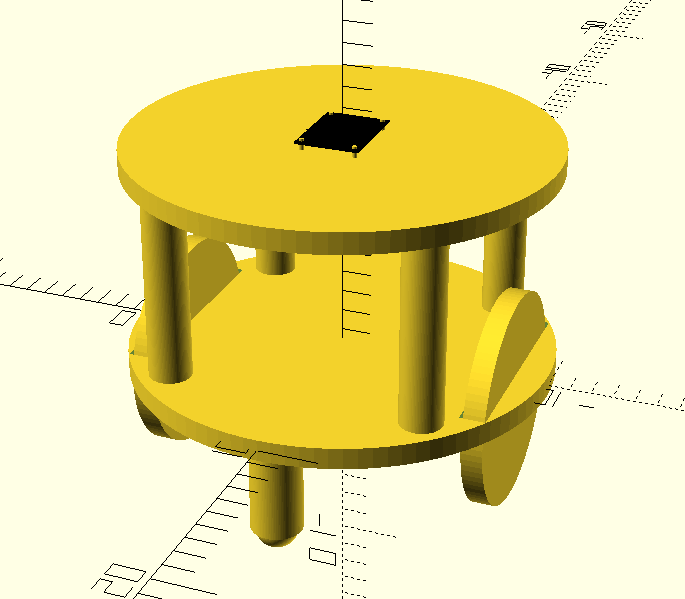
\includegraphics[scale=0.5]{figs/img/cleaningRobotModel7152020}
\end{figure}

\labday{Thursday, July 16, 2020}
To correct the problem of the robot getting removed after detecting for the first time, a rule will be set in place that the SBC must broadcast "iRobot Create 2". However, a \texttt{SocketTimeoutException} is still being thrown when the app attempts to receive data:
\begin{Verbatim}
2020-07-16 11:50:32.401 26129-26299/com.example.lidarmappingrobot 
I/MainActivity: IOException thrown in FindRobotTask
    java.net.SocketTimeoutException: Poll timed out
        at libcore.io.IoBridge.poll(IoBridge.java:691)
        at java.net.PlainDatagramSocketImpl.doRecv
        (PlainDatagramSocketImpl.java:149)
        at java.net.PlainDatagramSocketImpl.receive0
        (PlainDatagramSocketImpl.java:140)
        at java.net.AbstractPlainDatagramSocketImpl.receive
        (AbstractPlainDatagramSocketImpl.java:143)
        at java.net.DatagramSocket.receive(DatagramSocket.java:847)
        at com.example.lidarmappingrobot.MainActivity
        $FindRobotTask.run(MainActivity.java:148)
        at java.lang.Thread.run(Thread.java:764) /$
\end{Verbatim}
Further problems still exist as the robot listing disappears every time the view is refreshed. 
\medbreak\noindent
A pause was placed on the app to work on the Python program. Simply, a new thread is created for creating a TCP connection to the client after the IP address of the phone is retrieved. However, after running the lines:
\begin{Verbatim}
	ip = address[0]
	sock_obj = socket.socket(socket.AF_INET, socket.SOCK_STREAM)
	port = random.randint(20000, 50000)
	print(port)
	sock_obj.bind((ip,port))	
\end{Verbatim}
The \texttt{Cannot assign requested address} error is thrown. What I am trying to do is open up a direct connection between the app and robot. Since this method does not appear to work, I will simply write a server for the app that is constantly running and accepting connections. Then a new thread will be created for each subsequent connected device.

\labday{Friday, July 17, 2020}
I rewrote the Python program to have three different functions:
\begin{itemize}
\item \texttt{multicastListeningThread} which will simply listen for multicast messages from phones on group ('224.3.29.71', 10000)
\item \texttt{appListeningThread} which listens for phone connections by TCP once they have identified the SBC by a multicast request
\item \texttt{appCommunicationThread} which will be started when a new phone connects to the board and will process data sent by each phone. Each phone connected to the board will have its own \texttt{appCommunicationThread}.
\end{itemize}
Although the BeagleBone is the target platform for this program, I added another function called \texttt{gpioInit} which will set up the GPIO connections on the Raspberry Pi. 
\medbreak\noindent
In the \texttt{MapActivity} class of the app, I wrote an inner "task" class that implements \texttt{Runnable}

\labday{Tuesday, July 21, 2020}
A prototype of the UV disinfection device was worked on today. A possible change I would like to make is using Creo as a student license is available rather than OpenSCAD.

\labday{Wednesday, July 22, 2020}
Just to get a basic demonstration of app communication, I worked on getting communication between my app and the RPi working by toggling an LED on and off. In order to toggle a GPIO pin on and off with the \texttt{RPi.GPIO} library, the following code is used:
\begin{Verbatim}
GPIO.output(CHANNEL,GPIO.HIGH)
time.sleep(1)
GPIO.output(CHANNEL,GPIO.LOW)
time.sleep(1)
\end{Verbatim}
What will need to be determined is how to write strings through a socket in java. The following can be used for this purpose \footnote{\url{https://gist.github.com/chatton/8955d2f96f58f6082bde14e7c33f69a6}}:
\begin{Verbatim}
Socket socket = new Socket("localhost", 7777);
OutputStream dataOutputStream = socket.getOutputStream();
dataOutputStream.writeUTF("yo");
dataOutputStream.flush();
dataOutputStream.close();
\end{Verbatim}
The problem I am encountering is when strings get sent over from the app to the RPi, they contain non-ascii characters and unintended spaces upon arrival.

\labday{Friday, July 24, 2020}
From the meeting on Thursday:
\begin{itemize}
\item Design a place for the UV light emitter holder on the robot
\item Determine how to mount both the LIDAR sensor and the UV light
emitter together on the top plate of the robot
\item Focus majority of efforts for now on the app because the Roomba is what
will be worked on first
\end{itemize}
Today, some work was done on fixing the problem of the robot listing disappearing after refreshing. The problem I discovered is in the following code block:
\begin{Verbatim}[tabsize=4]
for(int i = 0; i < 10; i++) {
	DatagramPacket recv = new DatagramPacket(buf, buf.length);
	sock.receive(recv);
	ip = recv.getAddress().getHostAddress();
	recvMsg = new String(recv.getData(), 0, recv.getLength());

	if(recvMsg.equals("iRobot Create 2")) {
		// Check if the IP is already in the database or
		// is the local IP address
		if(!dbIps.contains(ip) && !ip.equals(localIpAddress)) {
			// Denote the IP address as a found IP
			foundIps.add(ip);

			// Construct a new Robot object and insert into the database.
			Robot robot = new Robot(recvMsg, ip);
			db.robotDao().insert(robot);
		}
		break;
	}
}

// Compare the foundIps and dbIps lists to check if there are any
// robots in dbIps that are not in foundIps. If so, remove it.
ArrayList<Robot> disconnectedRobots = new ArrayList<Robot>();
for(String dbIp : dbIps) {
	if(!foundIps.contains(dbIp)) {
		List<Robot> disconnectedRobotsTemp = db.robotDao().loadByIp(dbIp);
		disconnectedRobots.addAll(disconnectedRobotsTemp);
	}
}
\end{Verbatim}
Inside the for loop, the \texttt{foundIps} string array list is appended to only if there is not already a Robot containing the IP in the database and the IP is not the device's IP address. Simply by adding the line
\begin{Verbatim}
foundIps.add(ip); 
\end{Verbatim}
above the conditional statement
\begin{Verbatim}
if(recvMsg.equals("iRobot Create 2")
\end{Verbatim}
the problem of the device disappearing regularly after refreshing mostly was fixed. However, at times a socket timeout exception is thrown causing the device to disappear.
\medbreak\noindent
What needs to be done next is to determine how to pass the IP to the MapActivity through the \texttt{Intent} object. Quite simply, the \texttt{mRobotList} can be parsed to retrieve the correct IP by indexing the correct position of the arraylist. Then, this IP can be passed to the Intent with a call to \texttt{putExtra} and retrieved with \texttt{getStringExtra}. One of the problems I am encountering is that the app will crash when pressing the ON/OFF button in the map activity task due to a null reference exception.

\labday{Monday, July 27, 2020}
The null reference exception was fixed by correcting a reference to the \texttt{mIPAddress} class level variable by changing 
\begin{Verbatim}
String mIPAddress = intent.getStringExtra("ROBOT_IP");
\end{Verbatim}
to 
\begin{Verbatim}
mIPAddress = intent.getStringExtra("ROBOT_IP");
\end{Verbatim}
in the \texttt{onCreate} method of the \texttt{MapActivity} class. An LED was able to be succesfully toggled when clicking the ON/OFF button in the app. One of the potential problems is the fact that a small amount of delay occurs between when the button is pressed in the app and when the LED is toggled on or off. A second problem that needs to be solved is the exception:
\begin{Verbatim}[tabsize=4]
Exception in Thread-2:
Traceback (most recent call last):
	File "/usr/lib/python3.7/threading.py", line 917, in _bootstrap_inner
		self.run()
	File "/usr/lib/python3.7/threading.py", line 865, in run
		self._target(*self.args, **self._kwargs)
	File "receiver.py", line 46, in appListeningThread
		server_sock.bind('',APP_LISTENING_THREAD_PORT))
OSError: [Errno 98] Address already in use
\end{Verbatim}
This occurs when the program is interrupted with CTRL+C or in Python the KeyboardInterrupt. Somehow the server is not being shutdown properly when the program is interrupted. I attempted to add a try, except statement for the KeyboardInterrupt inside the while loop waiting for connections, but the problem still persisted. The main issue is likely that the superloop lies inside a thread. From StackOverflow~\footnote{\url{https://stackoverflow.com/questions/6380057/}}, a user suggests adding the line
\begin{Verbatim}
server_sock.setsockopt(socket.SOL_SOCKET, socket.SO_REUSEADDR, 1)
\end{Verbatim}
before binding. This issue occurs because the program containing the socket creation was executed too many times with too small of a delay between executions causing the socket to be left in a TIME\_WAIT state \footnote{\url{https://docs.python.org/3.3/library/socket.html}}. At this point the program is no longer throwing the above exception.

\labday{Tuesday, July 28, 2020}
Brian. Today some time was spent researching the pycreate2 python library that Jaden discovered\footnote{\url{https://github.com/MomsFriendlyRobotCompany/pycreate2}}. In order to drive the robot forward or backward or turn right or left, the \texttt{Create2.drive\_direct} method must be called with \texttt{r\_vel} or right wheel velocity and \texttt{l\_vel} or left wheel velocity passed as parameters. The velocity parameters are in mm/sec and clamped within the range (-500, 500) where -500 and 500 mm/sec are not included. Negative velocities denote rotation in the reverse direction while positive velocities denote rotation in the forward direction. This make it possible to turn the robot in place left or right, move backward, and forward. The user interface will have buttons for moving forward, backward, left and right. 

\labday{Wednesday, July 30, 2020}
Work was done on the app to control the robots movement. An initial step to this process was adding some code to the \texttt{receiver.py} program to allow connection and control of the robot over a serial connection. The constant speed of the robot will be set to 100 mm/sec. This value may need to be tweaked for steering speed. Some algorithms will need to be developed for allowing the robot to follow a pre-programmed path after hitting the submit button in the app. A maximum of 10 instructions (left, right, forward, backward) will be able to written to the robot at a given time. Next I worked on creating icons for each of the four buttons: left, right, upward, and downward arrows. The current issue I am having is the back button is not rendering properly to the display. Later the previously used \texttt{Button} views were altered to \texttt{ImageButton} objects for better image placement inside each button. These problems were fixed after removing the bottom constraints of each of the buttons. This layout will need to be switched to another layout corresponding to the \texttt{ControlActivity} which I will need to create for manually controlling the robot's movement.

\labday{Monday, August 3, 2020}
I added a new \texttt{Activity} class titled \texttt{ControlActivity} which will handle sending queues of control commands to the robot. Instead, a different approach was taken where two tabs titled Map and Control will be added. One of the problems I am trying to solve is how to associate a layout file with a \texttt{TabItem} view. The following code can be used to get a tab item at a position and configure it with a layout file:
\begin{Verbatim}
TabLayout tabLayout = (TabLayout) findViewById(R.id.tabs);
TabLayout.Tab tab = tabLayout.getTabAt(1);

tab.setCustomView(R.layout.activity_map);
\end{Verbatim}
However, I do not know how to write a fragment for a given tab. I looked through the blog post \footnote{\url{https://www.techotopia.com/index.php/Creating_an_Android_Tabbed_Interface_using_the_TabLayout_Component}}. Essentially in the \texttt{DiscoveryArrayAdapter} which sets on a \texttt{setOnClickListener} for the \texttt{RecyclerView}. Inside the click listener, it should activate a new activity titled \texttt{BaseRobotActivity}. The layout inflated in this activity will include two tabs titled \texttt{Map} and \texttt{Control}. In order to set fragments for each of these tabs, a subclass of \texttt{FragmentPagerAdapter} must be written. 
\medbreak\noindent
However, from an email from Dr. Miah, the focus will now shift to working on the new robot prototype.

\labday{Tuesday, August 4, 2020}
I worked on researching current UV disinfecting robot designs. All of the ones I have seen seem to have very long UV lamps mounted on top that will shine around the room. Possibly, a LIDAR sensor can be mounted on top of the UV lamps.

\labday{Wednesday, August 5, 2020}
In the design, I would also like to have four wheels with front and back sets of wheels steerable via servo for precise rotation and control. Axles will connect the front and back sets of wheels together. This does have pros and cons as having large wheels will likely help with stability and prevent the robot from toppling over if it is nudged or bumped. However, one of the downsides of the design is a less tight turning radius. For now I will work on learning how to use Creo as I decided to switch to this as OpenSCAD is very limited in terms of features and Creo is a professional CAD modeling software where precise dimensions may be specified. The first tutorial I worked on was a car piston. Work was started on modeling the chassis of the robot which simply consists of a rectangular box which will house the wheels, steering system, and electronics like the single board computer and motor drivers. However, a rectangular box may not look appealing to the eye. Since changes are still being made to the design, I decided to do away with having four wheels and two sets of steering servos. Rather two wheels will be used for controlling the movement and two caster wheels. In this way, the robot can have full 360 degree rotation; however, it may not be as stable. I designed a 1.5 ft by 1 ft essentially rectangular box that will act as the first layer of the robot which will house the motors/wheels and caster wheels.

\labday{Saturday, August 8, 2020}
Amr and I met yesterday and decided to go design a differential drive robot which will consist of two driveable/controllable wheels mounted under the middle of the base and two caster wheels at the front and back mounted under the base. Because 16 sonar/ultrasonic sensors are required, the shape of the robot base will be circular rather than rectangular. One of the first tasks after working on is the caster wheels. 

\labday{Monday, August 10, 2020}
One of the problems I need to solve is where to place the LIDAR sensor on top of the middle section of the robot. Placing it on top of the UV lamp stack may be problematic as it will be greater than 3 ft above the ground.

\labday{Wednesday, December 23, 2020}
 Added Nicolaus Shepard to the project. Redesigned the robot body from scratch now in Fusion 360. Trying out a hing design to minimize the space taken up buy the UV lights. We also need to add an electrostatic sprayer which will be tricky given the limited amount of space on the top of the robot.

\labday{Thursday, December 24, 2020}
\experiment{Meeting minutes}
Some of the takeaways from the meeting:
\begin{itemize}
\item Find link from UV light presented in meeting with Globex health
\item Prismatic joint to be used for UV light to retract into the body of the robot
\item Disinfectant liquid should be stored in the chassis
\item Mount for sprayer designed from scratch, use existing sprayer on the market
\item 9.25 cm wheel radius
\item For now only design a mount that will adjust the azimuth angle of the sprayer
\item Share the Android app repository with Nicholas
\end{itemize}
\experiment{Lab work}
Nicholas and I continued to work on the body design. Nicholas enlarged the wheels to 9.25 cm in radius. He added a prismatic joint conveyor belt system to allow the light to move up and down out of the robot chassis. I added a holder for the sprayer nozzle which we are to hopefully purchase off Amazon if time allows. A stepper motor will be used to control the azimuth angle of the sprayer. It will only have around 180 degrees of range for now. Nicholas continued to work on the caster wheel on the back of the robot to support the larger wheel size.

\labday{Monday, December 28, 2020}
\experiment{Laboratory work}
BL\\
I worked on adding finding motors to drive the motors today as this is necessary in case adjustments need to be made to the size of the robot chassis to account for the disinfectant tank.

\labday{Monday, January 4, 2021}
\experiment{Laboratory work}
BL\\
The robot drive wheels have part number 6331K31 on the McMaster-Carr website which I will need to show to Dr. Miah in case they are too expensive at a price of \$122.05 per unit. The problem with using a UV lamp setup is the fact that UV lamps often solely use 120 V AC which be expensive and difficult to implement as many batteries will be needed to support this continuous power delivery. Dr. Miah mentioned that it is okay to have really expensive dc motors in the design currently and we need to find a way to make a universal mount for the sprayer and UV light. Some pictures of the current robot and its components are pictured below
\begin{figure}[H]
\begin{subfigure}{.5\textwidth}
\centering
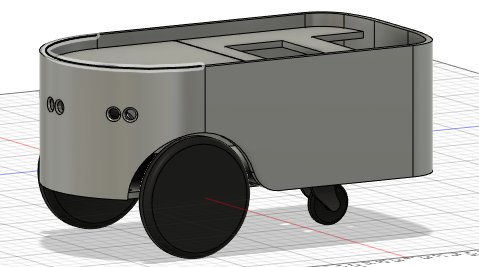
\includegraphics[scale=0.5]{figs/img/v2BodyDesign}
\subcaption{Body design}
\end{subfigure}
\begin{subfigure}{.5\textwidth}
\centering
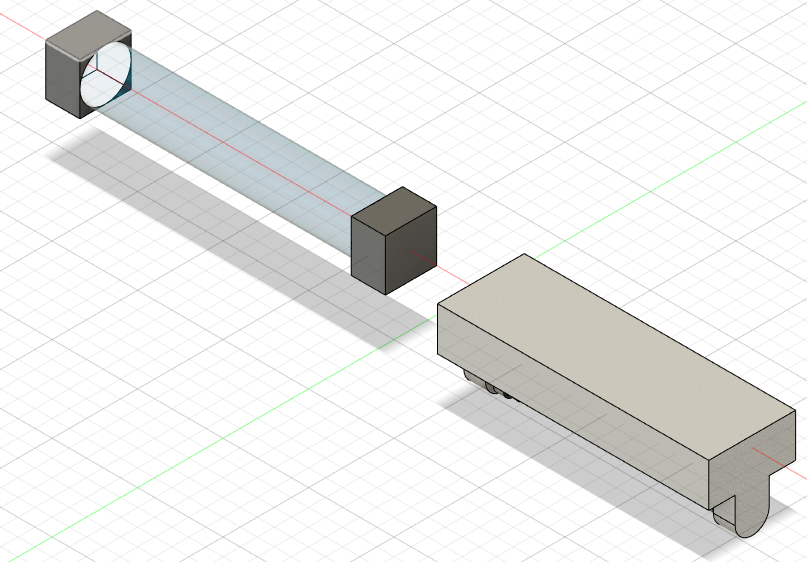
\includegraphics[scale=0.3]{figs/img/v2UVLamp}
\subcaption{UV lamp model}
\end{subfigure}
\begin{subfigure}{.5\textwidth}
\centering
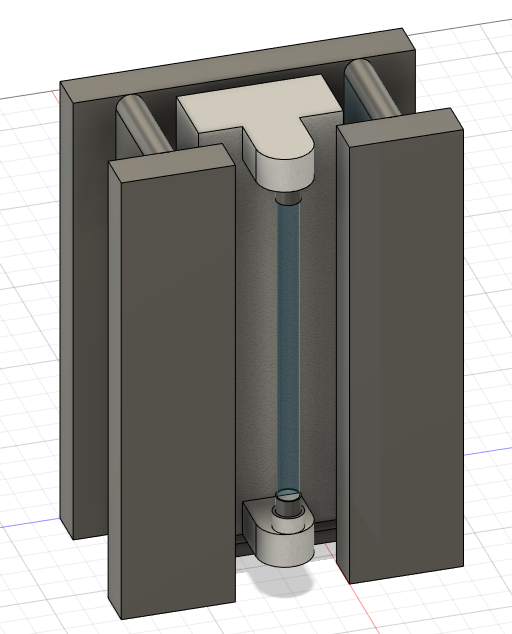
\includegraphics[scale=0.3]{figs/img/v2UVLampConveyor}
\subcaption{UV lamp conveyor}
\end{subfigure}
\begin{subfigure}{.5\textwidth}
\centering
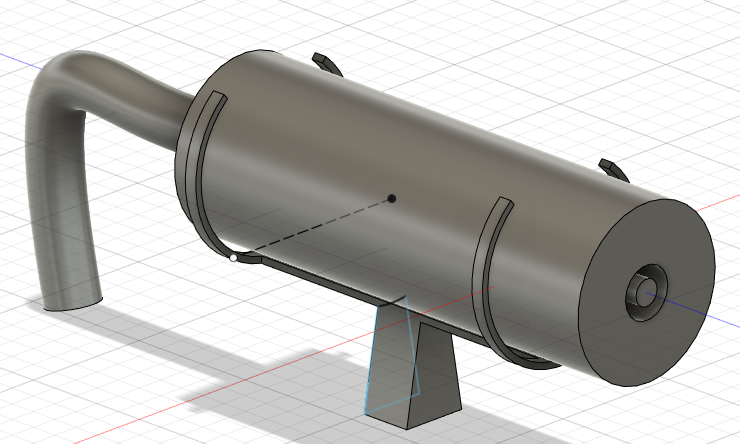
\includegraphics[scale=0.3]{figs/img/v2SprayerMount}
\subcaption{Disinfectant sprayer mount}
\end{subfigure}
\end{figure}
We still need to redesign the sprayer mount and UV light holder to be able to hold many different types of UV lights and disinfectant sprayers.
\end{addmargin} 

%----------------------------------------------------------------------------------------
%	BIBLIOGRAPHY
%----------------------------------------------------------------------------------------

\bibliography{bib/cam.bib}
\bibliographystyle{plain}
%----------------------------------------------------------------------------------------

\end{document}
%%% Local Variables:
%%% mode: latex
%%% TeX-master: t
%%% End:
